%
% Switches
%
% Aleph Objects Firewall
%
% Copyright (C) 2014, 2015, 2016 Aleph Objects, Inc.
%
% This document is licensed under the Creative Commons Attribution 4.0
% International Public License (CC BY-SA 4.0) by Aleph Objects, Inc.
%

\section{Overview}
There are now many new free software solutions for network switches.
Unfortunately, they are all high-end data center gear, the least expensive
costing over \$3,000USD.

\section{Open Compute Project}
http://www.opencompute.org/  http://github.com/opencomputeproject

\begin{figure}[h!]
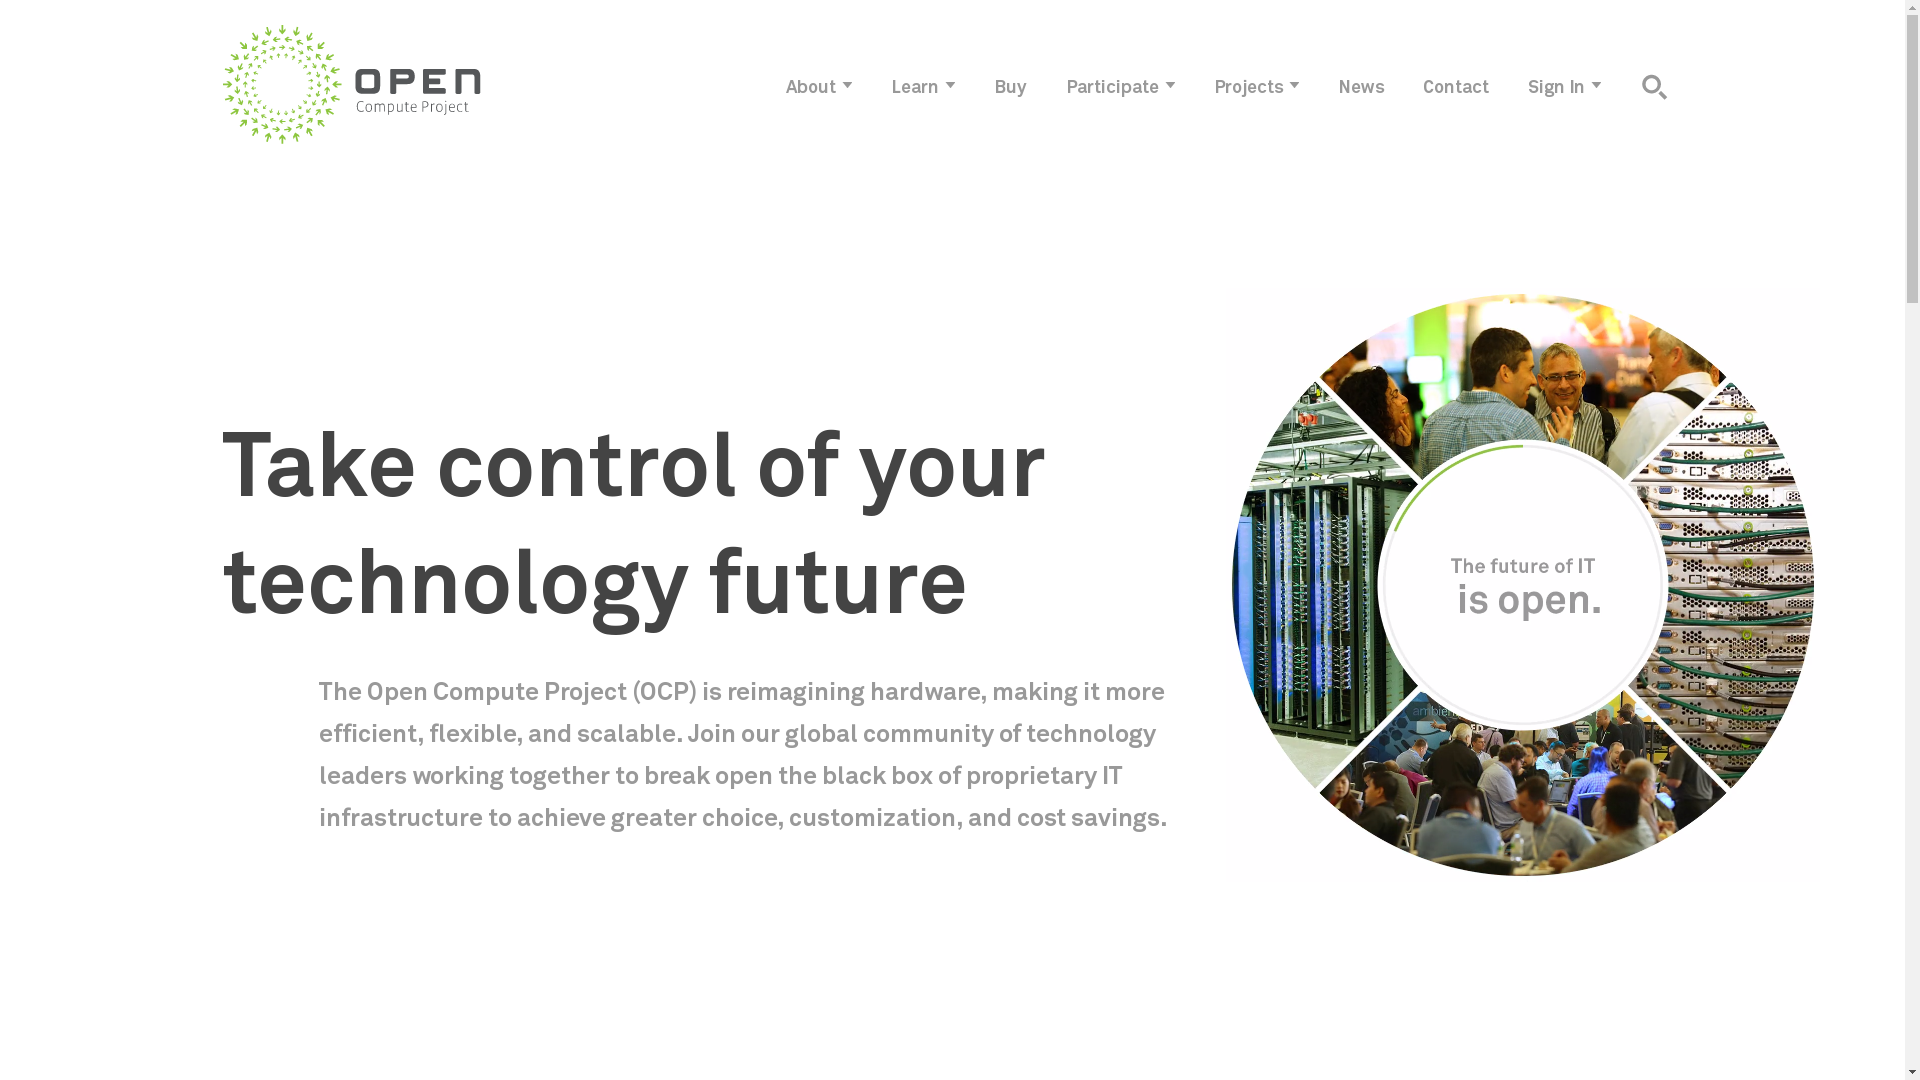
\includegraphics[keepaspectratio=true,height=1.10\textheight,width=1.00\textwidth,angle=0]{www-opencompute.png}
 \caption{OpenCompute Website}
 \label{fig:www-opencompute}
\end{figure}


Project so massive data centers can be more "open" and interoperate better
between vendors, by using free software.


\section{ONIE}
``The Open Network Install Environment (ONIE) is an Open Compute Project open source initiative driven by a community to define an open ``install environment'' for bare metal network switches, such as existing ODM switches and the upcoming OCP Network Switch design. ONIE enables a bare metal network switch ecosystem where end users have a choice among different network operating systems.... ONIE was contributed to the Open Compute Project.... ONIE is an open source ``install environment'', that acts as an enhanced boot loader utilizing facilities in a Linux/BusyBox environment. This small Linux operating system allows end-users and channel partners to install the target network OS as part of data center provisioning, in the fashion that servers are provisioned.''


Website: http://onie.org

Source code: https://github.com/opencomputeproject/onie

Wiki: https://github.com/opencomputeproject/onie/wiki

License: GPLv2

Hardware status: \url{http://www.opencompute.org/wiki/Networking/ONIE/HW_Status}

Operating System Support: \url{http://www.opencompute.org/wiki/Networking/ONIE/NOS_Status}

\begin{figure}[h!]
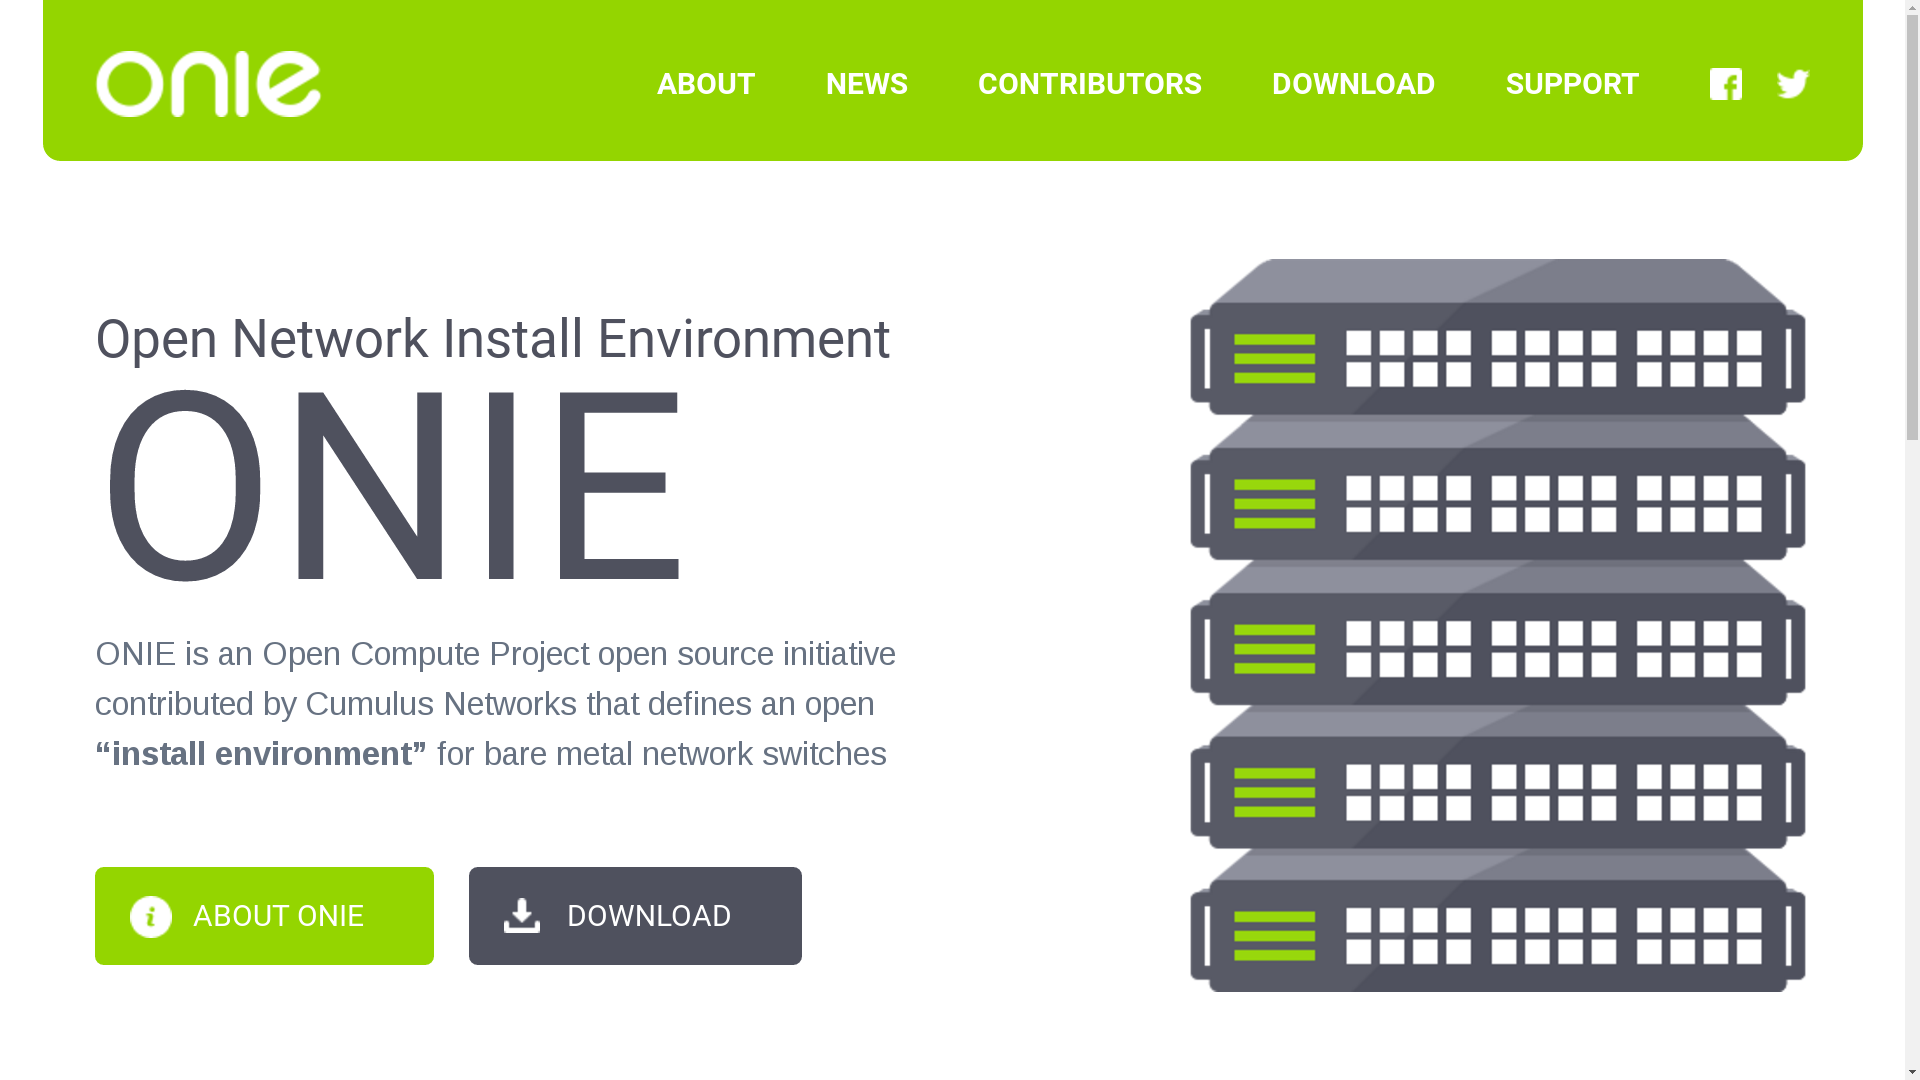
\includegraphics[keepaspectratio=true,height=1.10\textheight,width=1.00\textwidth,angle=0]{www-onie.png}
 \caption{ONIE Website}
 \label{fig:www-onie}
\end{figure}


\section{Switch Operating Systems}

\subsection{Open Network Linux}
opennetlinux.org
Distro for bare metal switches.

https://opennetlinux.org/

\begin{figure}[h!]
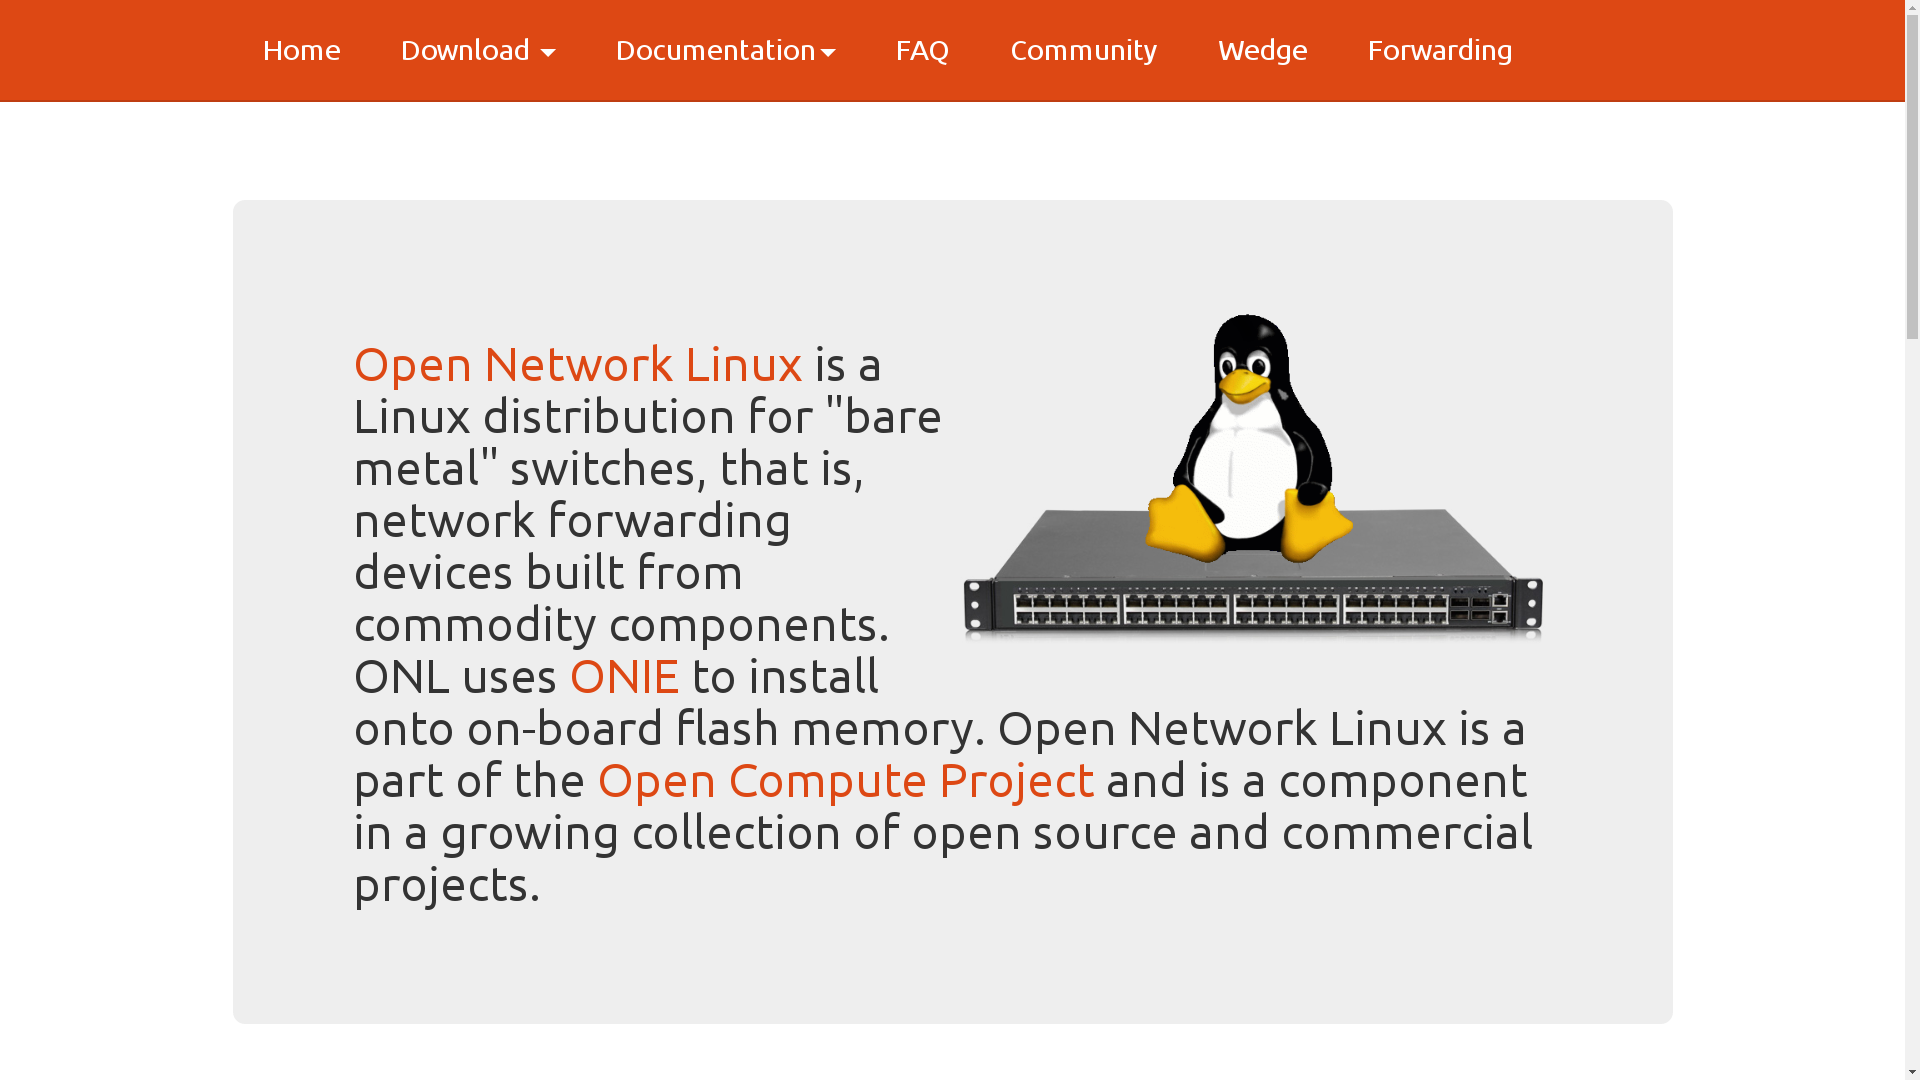
\includegraphics[keepaspectratio=true,height=1.10\textheight,width=1.00\textwidth,angle=0]{www-onl.png}
 \caption{Open Network Linux Website}
 \label{fig:www-onl}
\end{figure}


\subsection{Snaproute}
aka OpenSnaproute, FlexSwitch

http://www.snaproute.com/

https://opensnaproute.github.io/docs/

\begin{figure}[h!]
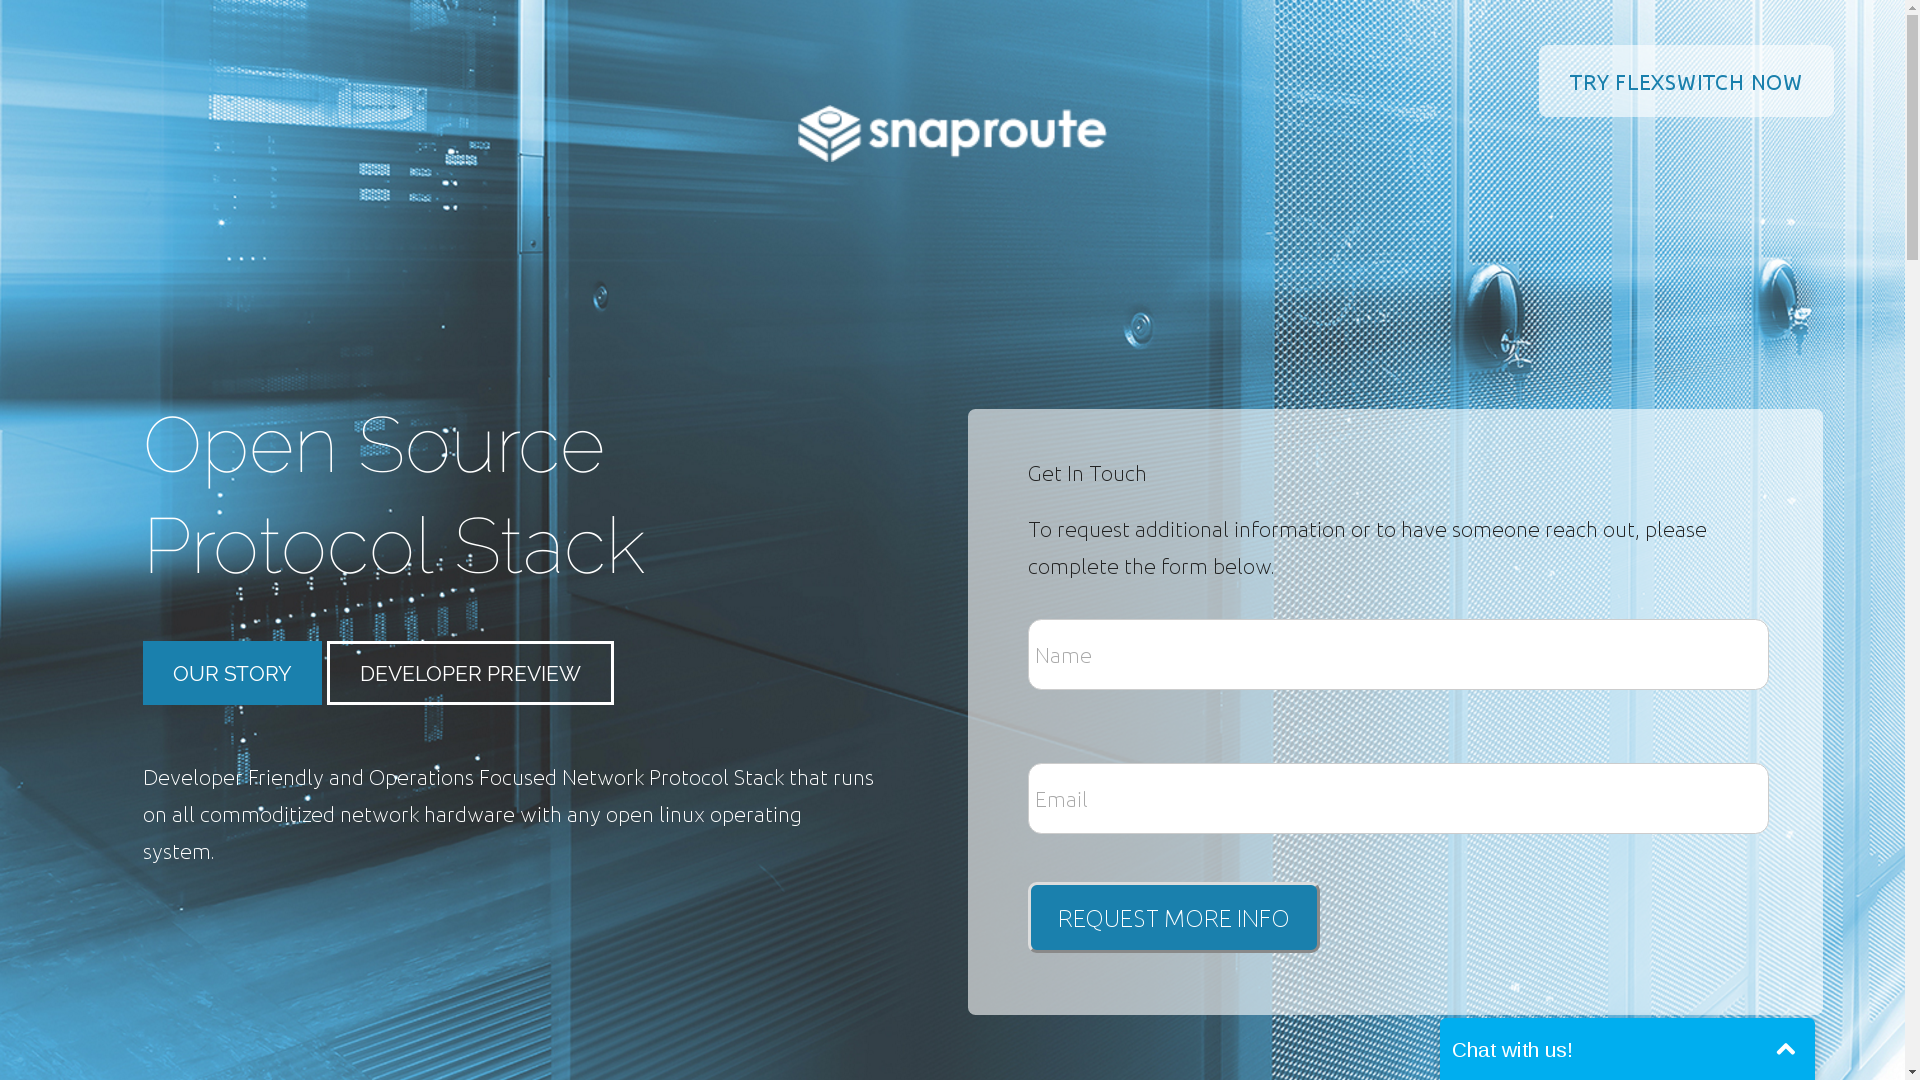
\includegraphics[keepaspectratio=true,height=1.10\textheight,width=1.00\textwidth,angle=0]{www-snaproute.png}
 \caption{Snaproute Website}
 \label{fig:www-snaproute}
\end{figure}


\subsection{OpenSwitch}

http://www.openswitch.net/

\begin{figure}[h!]
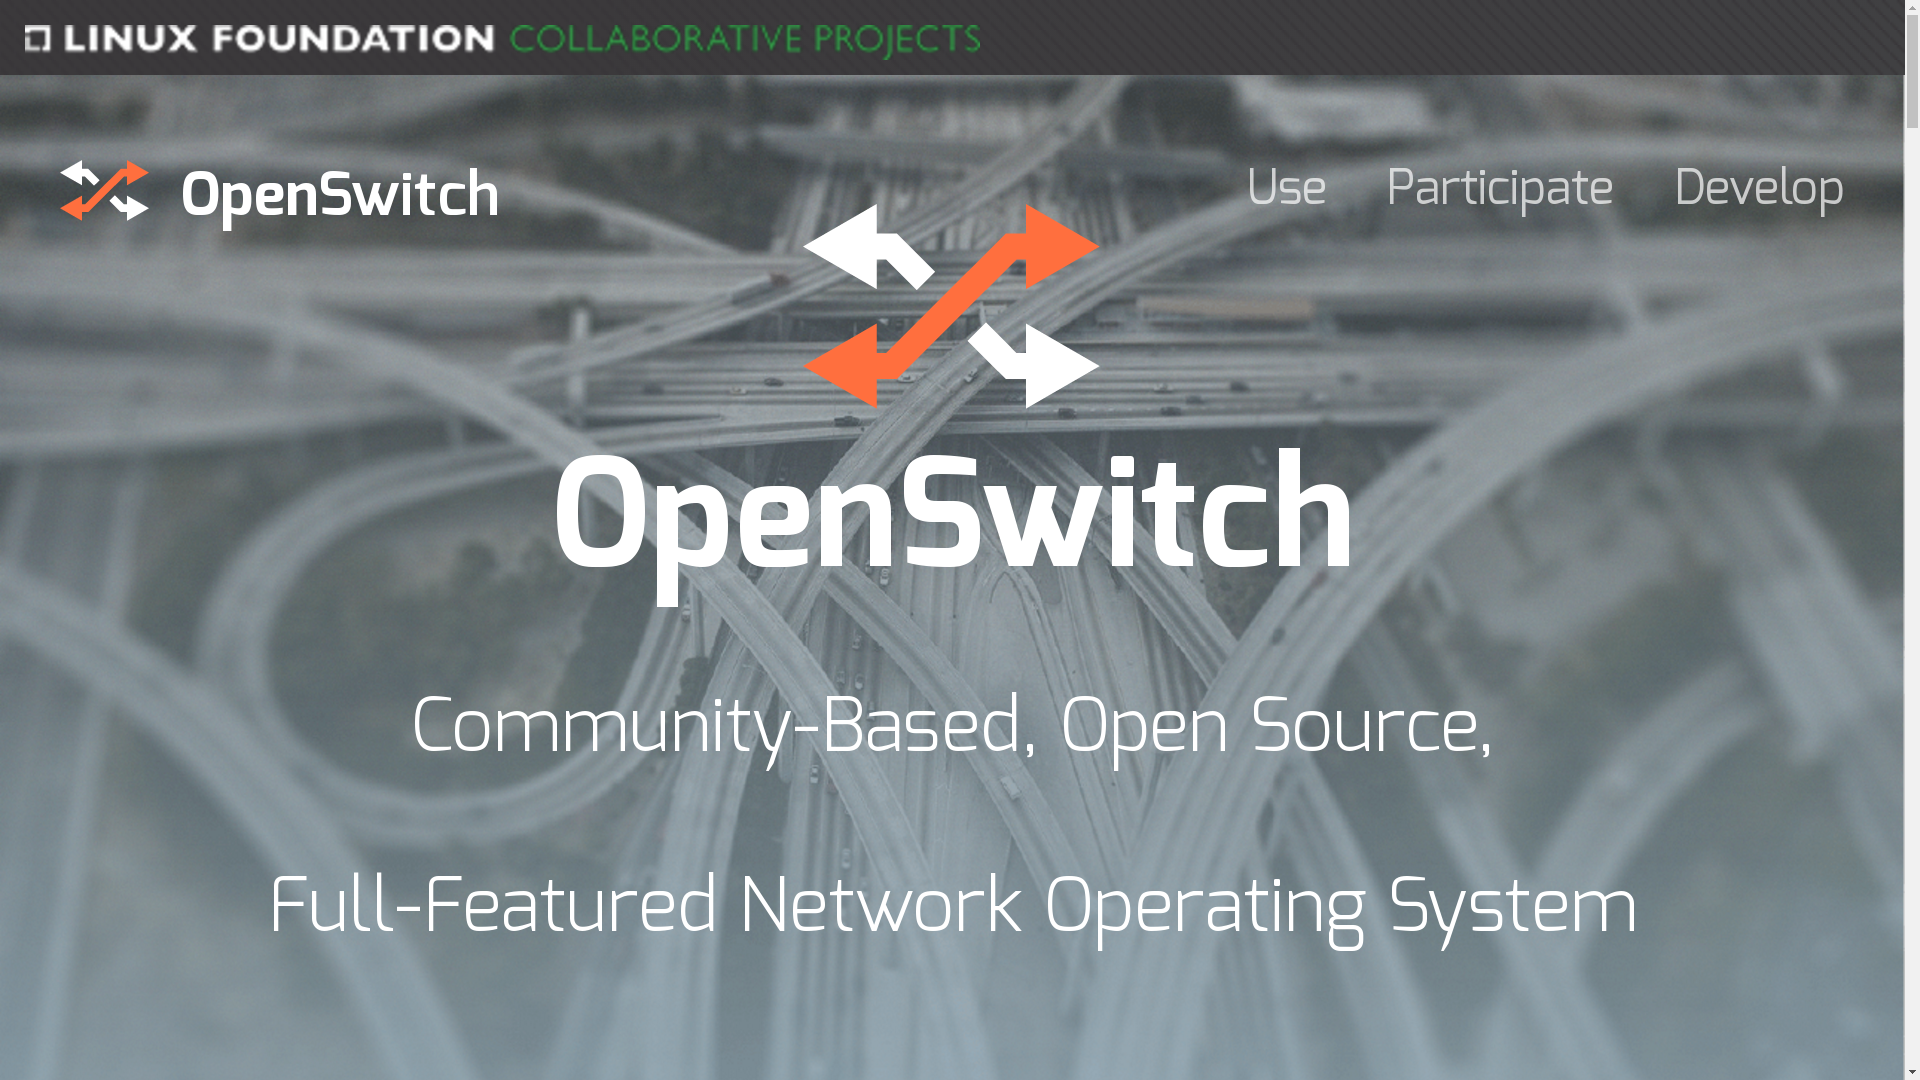
\includegraphics[keepaspectratio=true,height=1.10\textheight,width=1.00\textwidth,angle=0]{www-openswitch.png}
 \caption{OpenSwitch Website}
 \label{fig:www-openswitch}
\end{figure}


\subsection{FBOSS}

https://github.com/facebook/fboss

\begin{figure}[h!]
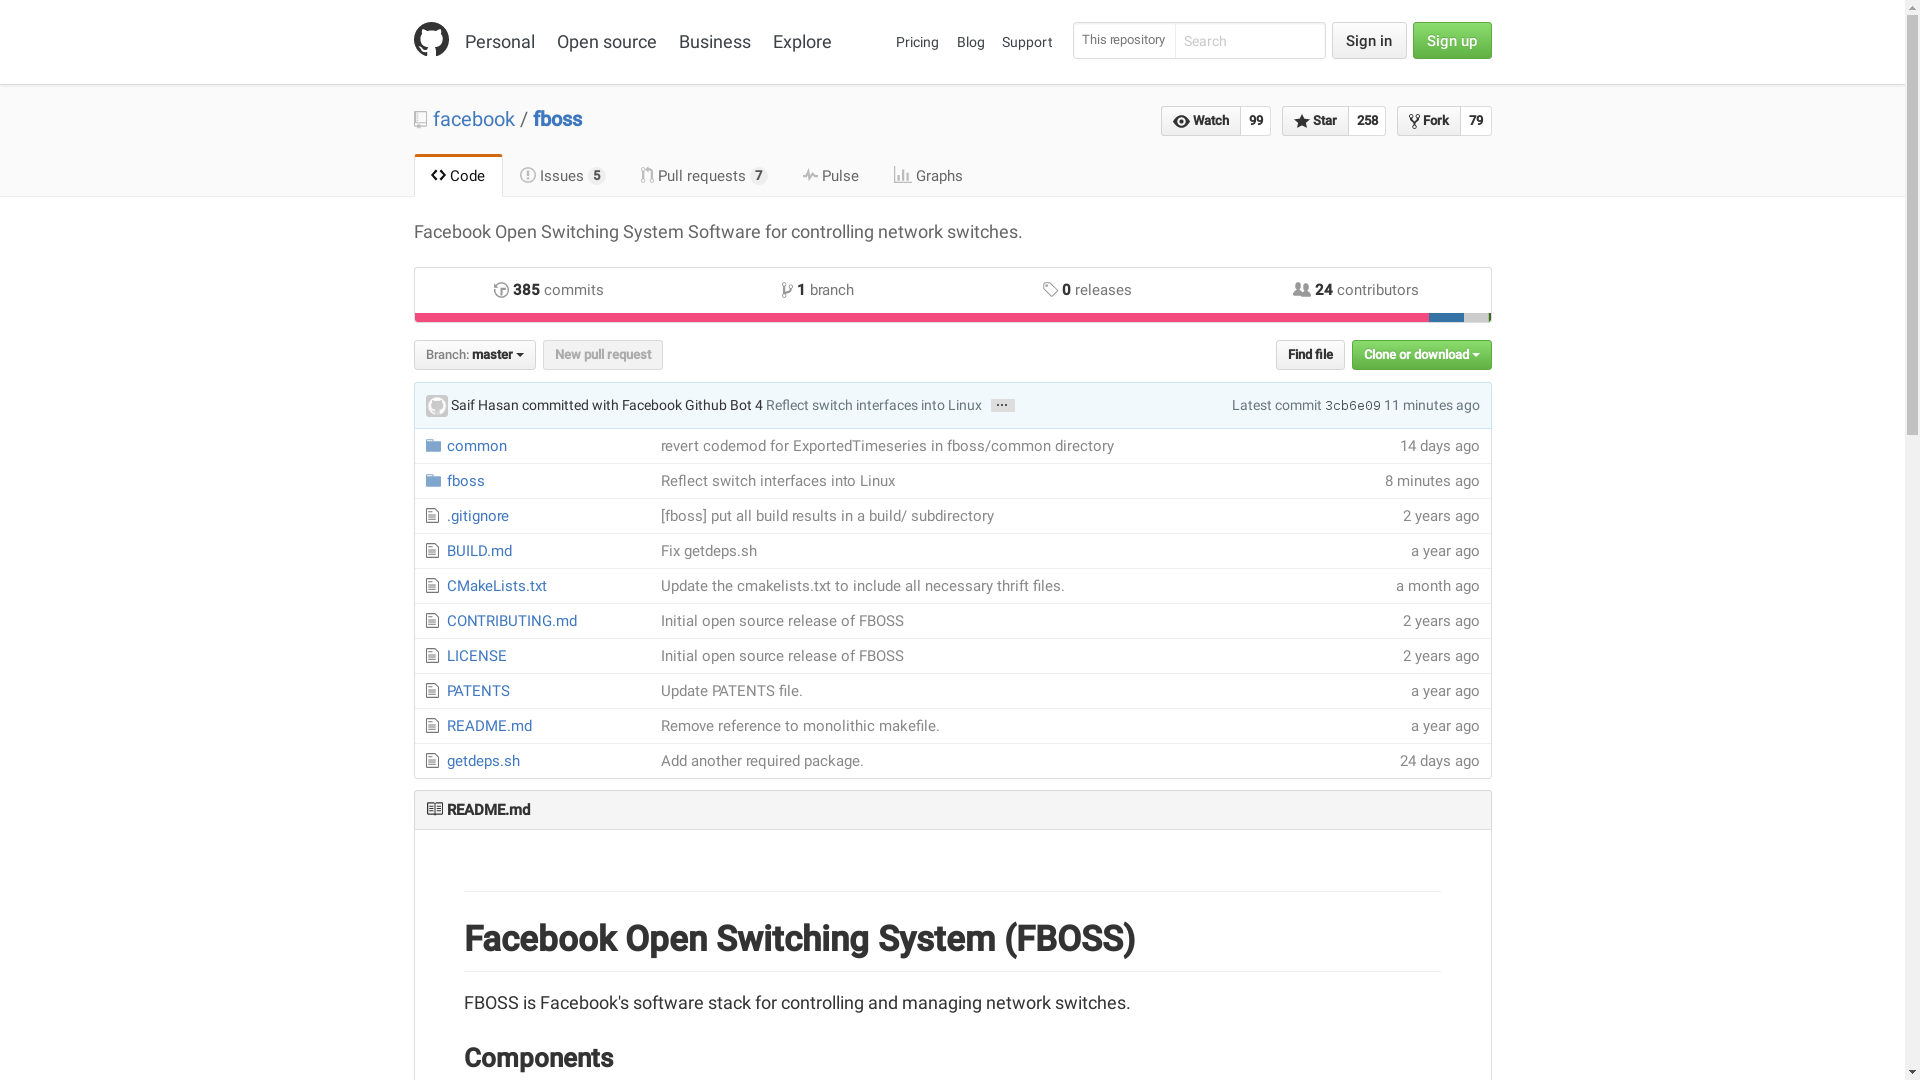
\includegraphics[keepaspectratio=true,height=1.10\textheight,width=1.00\textwidth,angle=0]{www-fboss.png}
 \caption{FBOSS Website}
 \label{fig:www-fboss}
\end{figure}


\subsection{Big Switch}

http://www.bigswitch.com/community-edition

Looks like baitware. Crippled version.

\begin{figure}[h!]

\includegraphics[keepaspectratio=true,height=1.10\textheight,width=1.00\textwidth,angle=0]{www-bigswitch.png}
 \caption{Big Switch Website}
 \label{fig:www-bigswitch}
\end{figure}


\section{Misc}

\begin{itemize}
 \item OpenNSL -- Broadcom chipsets. Accton. Github archive has proprietary
   license (LICENSE-Adv = non-free).
 \item OF-DPA -- From Broadcom.
 \item SAI 
\end{itemize}


Forwarding Agents
\begin{itemize}
 \item Quagga -- http://www.quagga.net/
 \item BIRD -- http://bird.network.cz/
 \item Azure SONiC
\end{itemize}


\section{Hardware}

\subsection{Edge-Core}
Edge-Core -- \url{http://www.edge-core.com/} -- Owned by Accton.

\begin{figure}[h!]
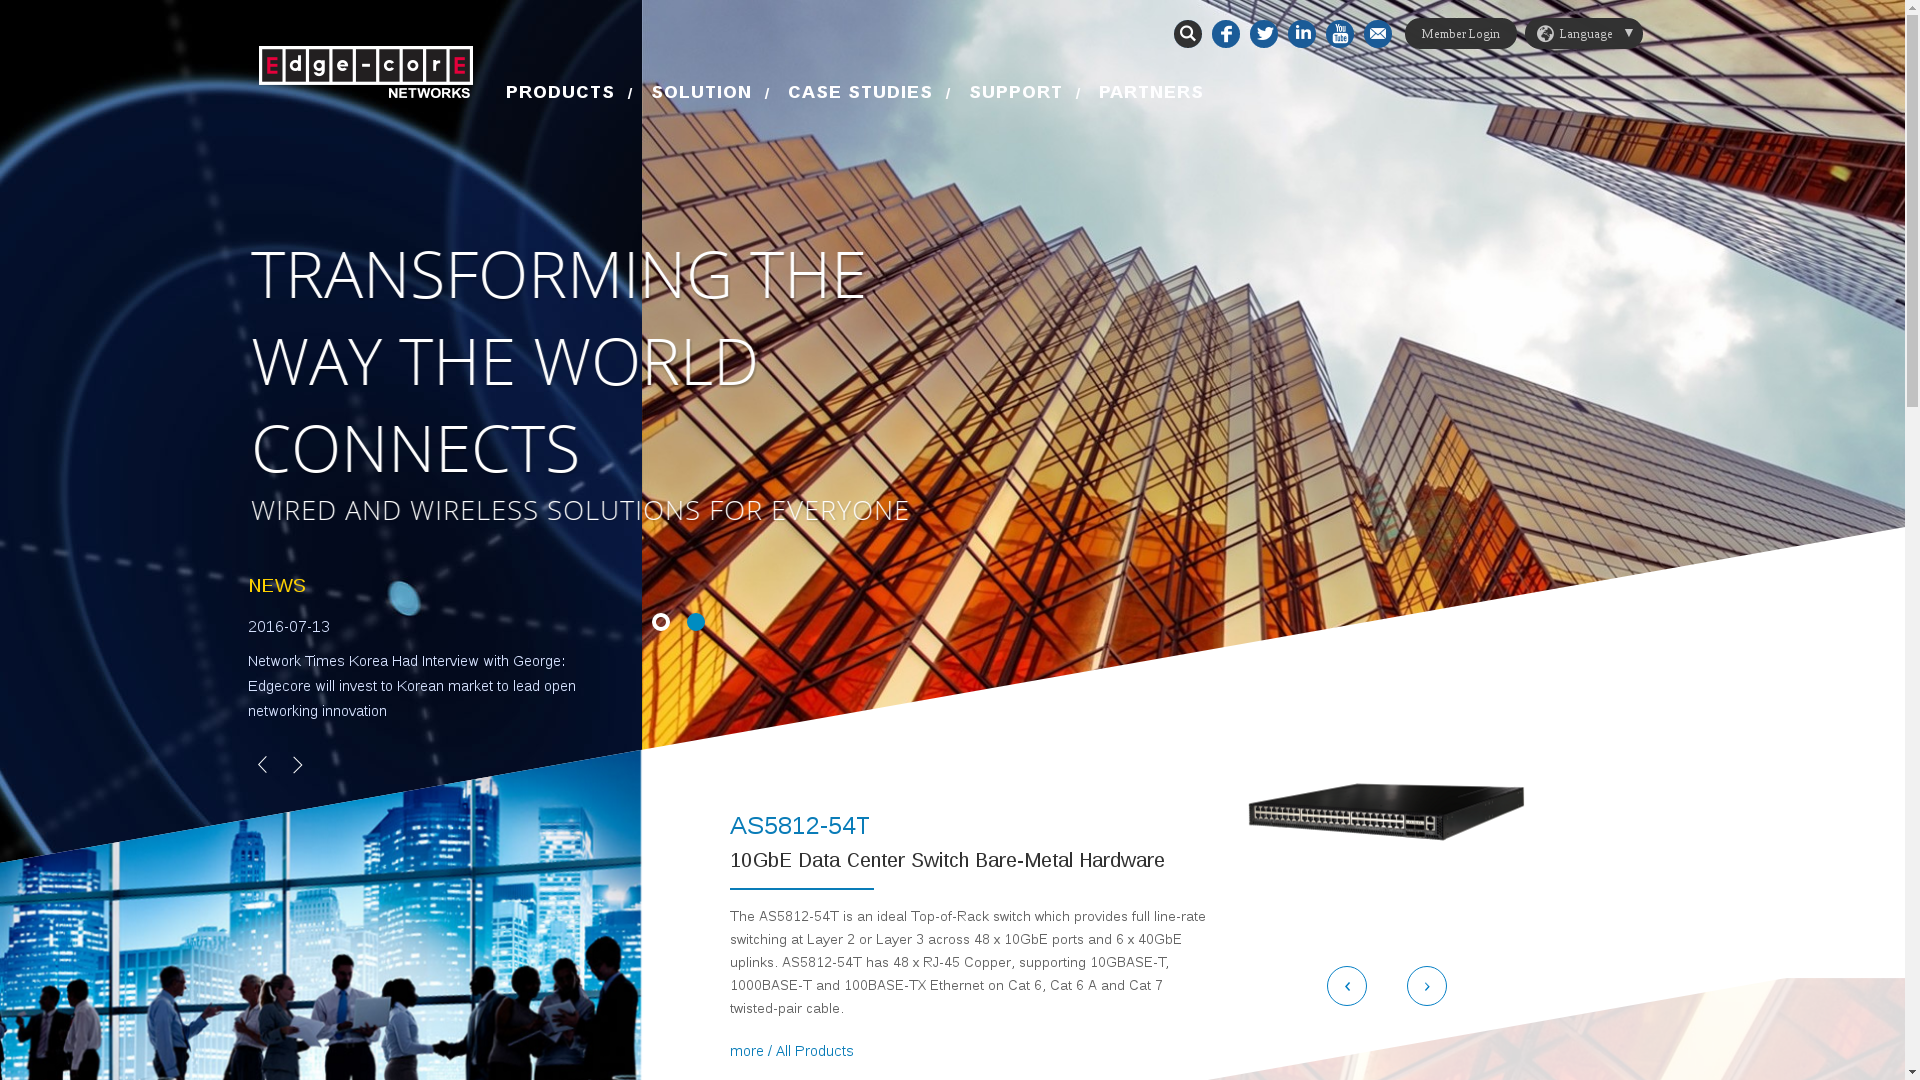
\includegraphics[keepaspectratio=true,height=1.10\textheight,width=1.00\textwidth,angle=0]{www-edge-core.png}
 \caption{Edge-core Website}
 \label{fig:www-edge-core}
\end{figure}


\subsection{Dell}


\subsection{Netberg}

\begin{figure}[h!]
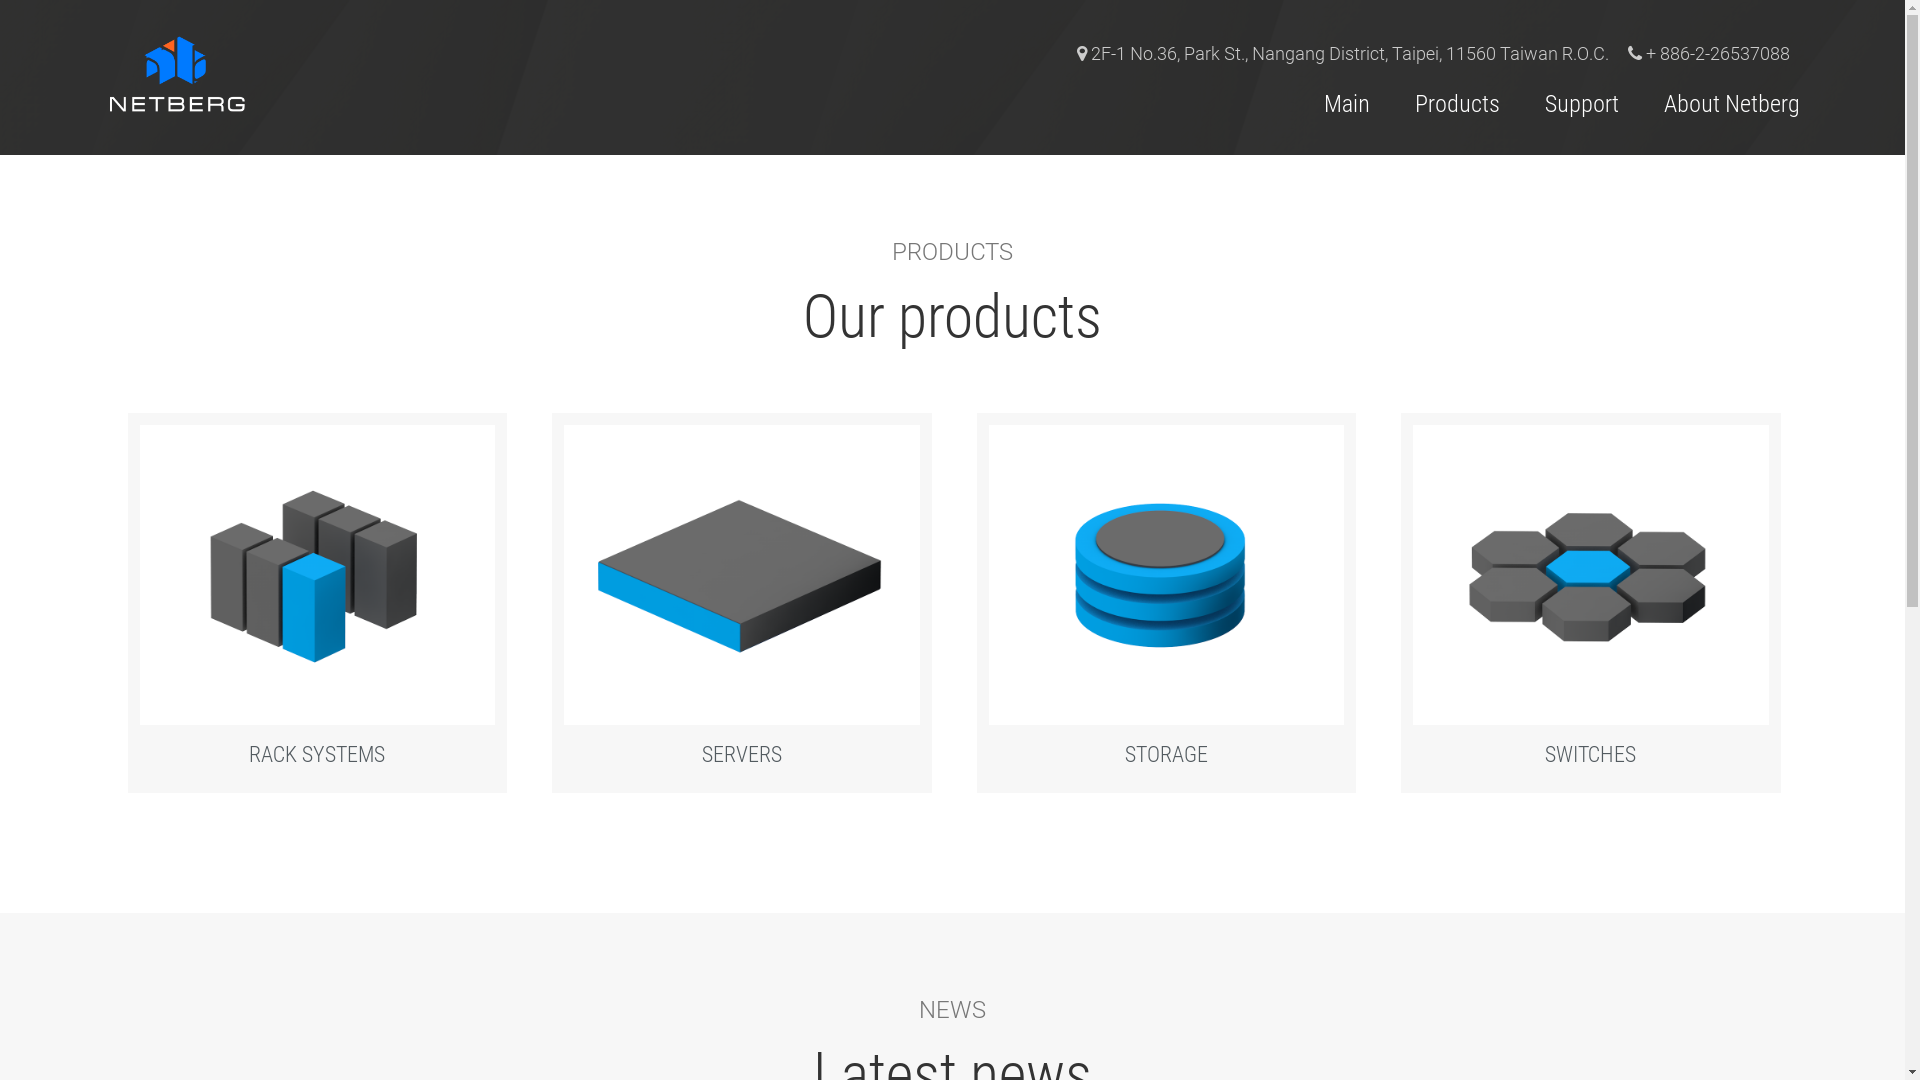
\includegraphics[keepaspectratio=true,height=1.10\textheight,width=1.00\textwidth,angle=0]{www-netberg.png}
 \caption{Netberg Website}
 \label{fig:www-netberg}
\end{figure}


\subsection{Quanta}

\begin{figure}[h!]
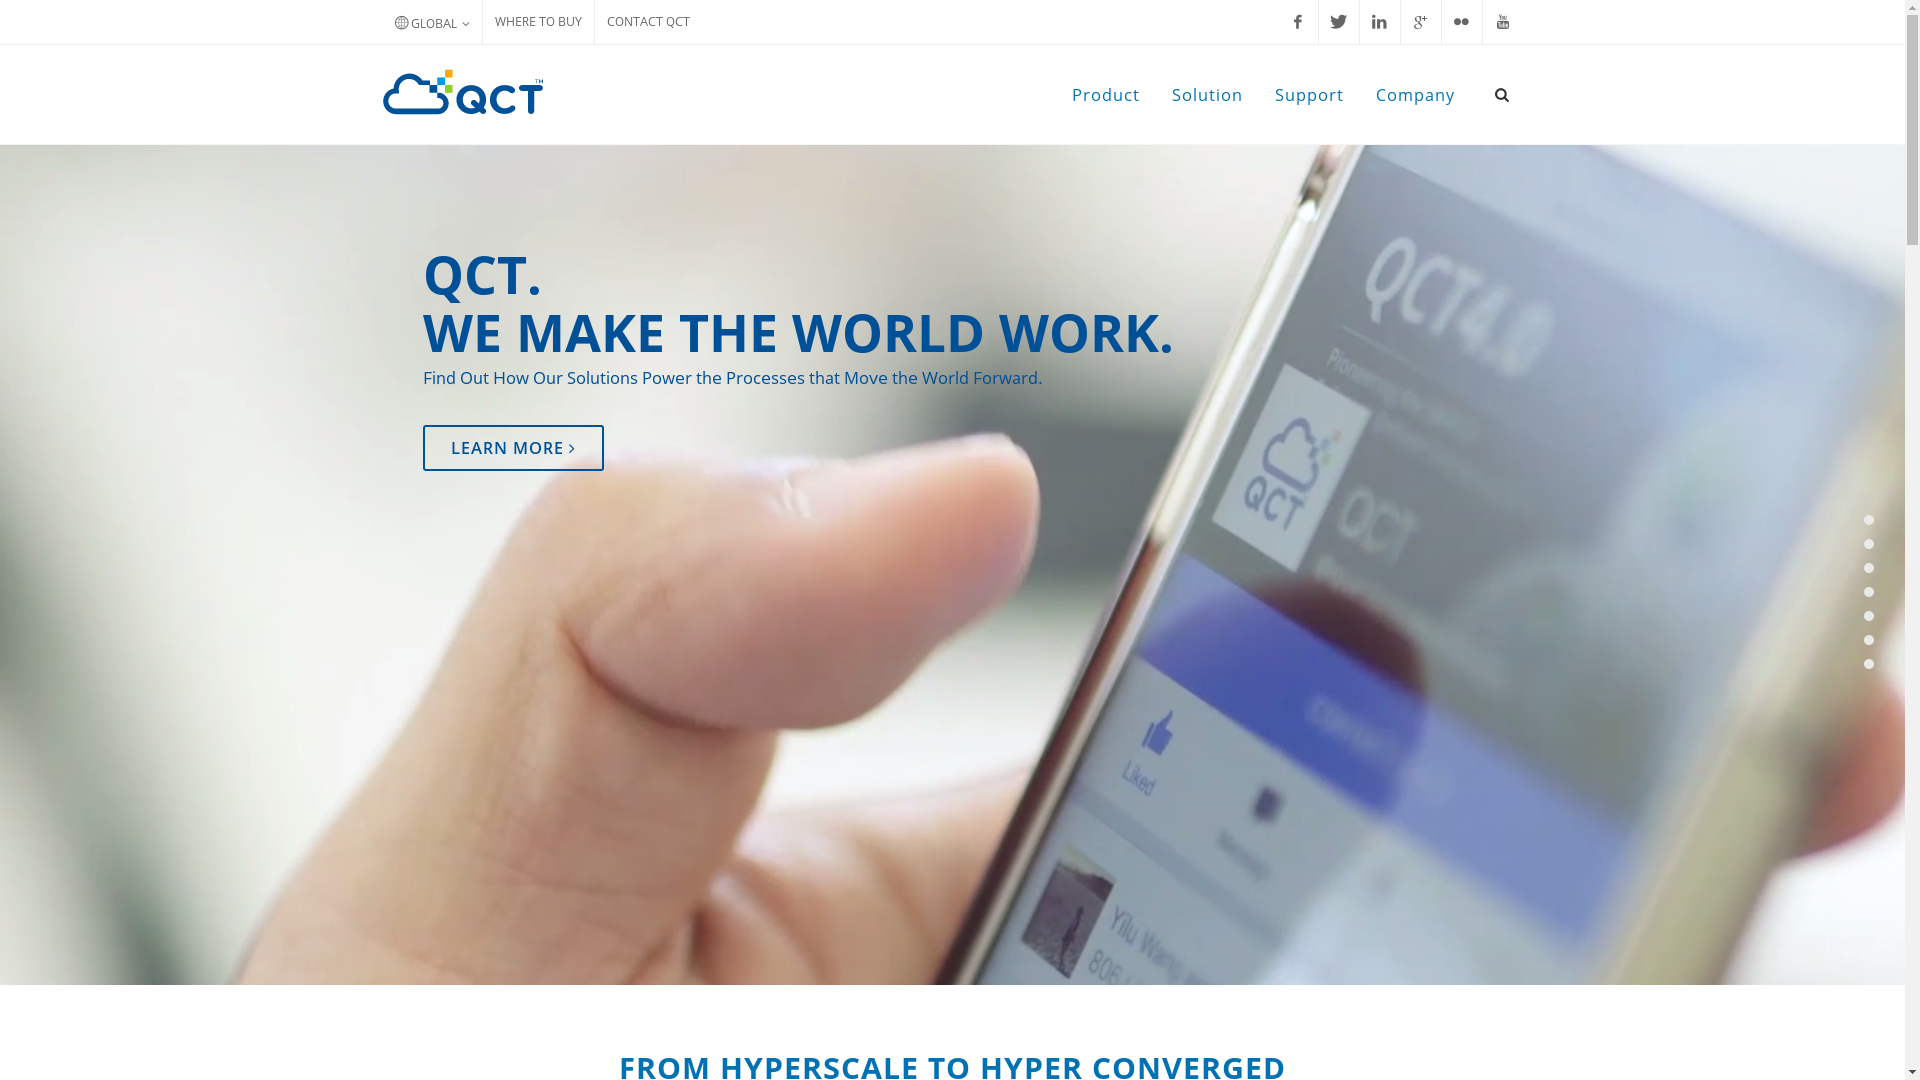
\includegraphics[keepaspectratio=true,height=1.10\textheight,width=1.00\textwidth,angle=0]{www-quanta.png}
 \caption{Quanta Website}
 \label{fig:www-quanta}
\end{figure}


\section{Suppliers}

\subsection{White Box}
White Box -- \url{http://whiteboxswitch.com/} -- Reseller of open switches.

\begin{figure}[h!]
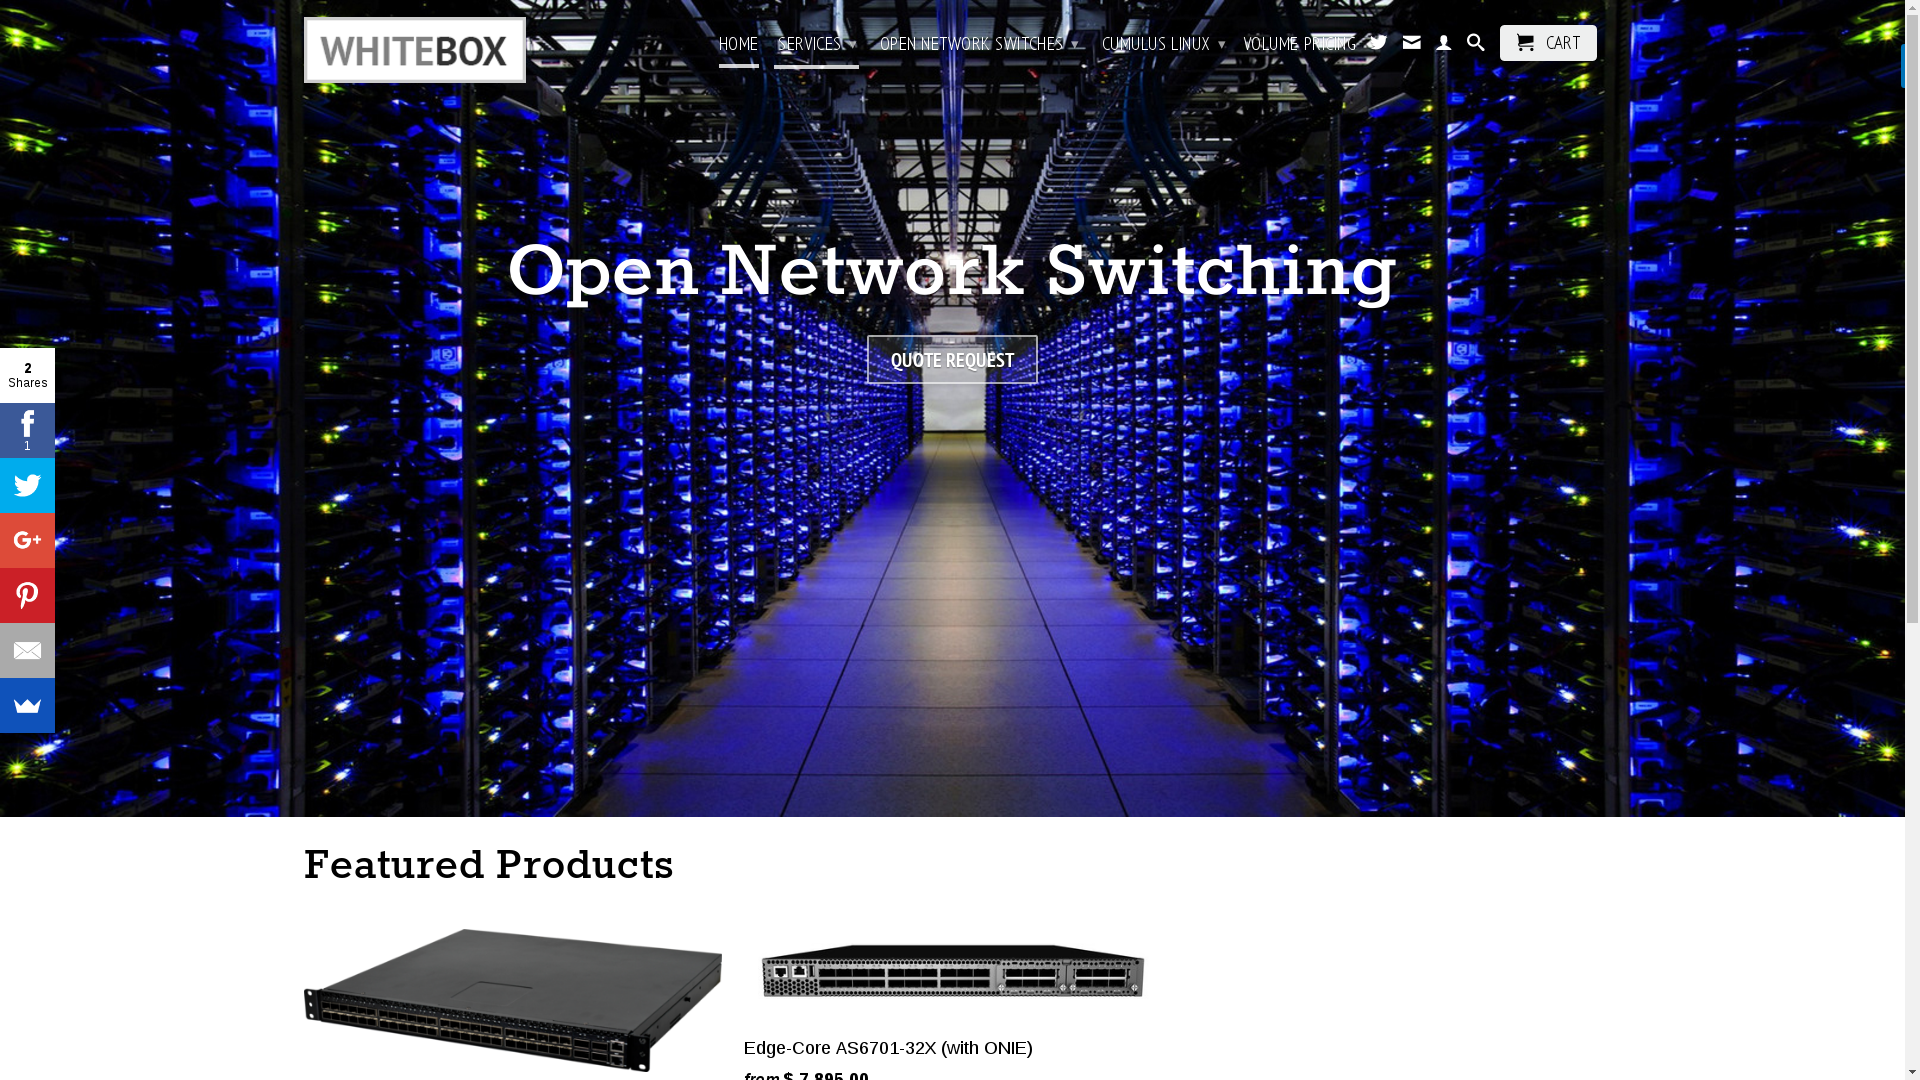
\includegraphics[keepaspectratio=true,height=1.10\textheight,width=1.00\textwidth,angle=0]{www-whitebox.png}
 \caption{Whitebox Website}
 \label{fig:www-whitebox}
\end{figure}


\subsection{Bare Metal Switches}
Bare Metal Switches -- \url{https://bm-switch.com/} -- Reseller of open switches.

\begin{figure}[h!]
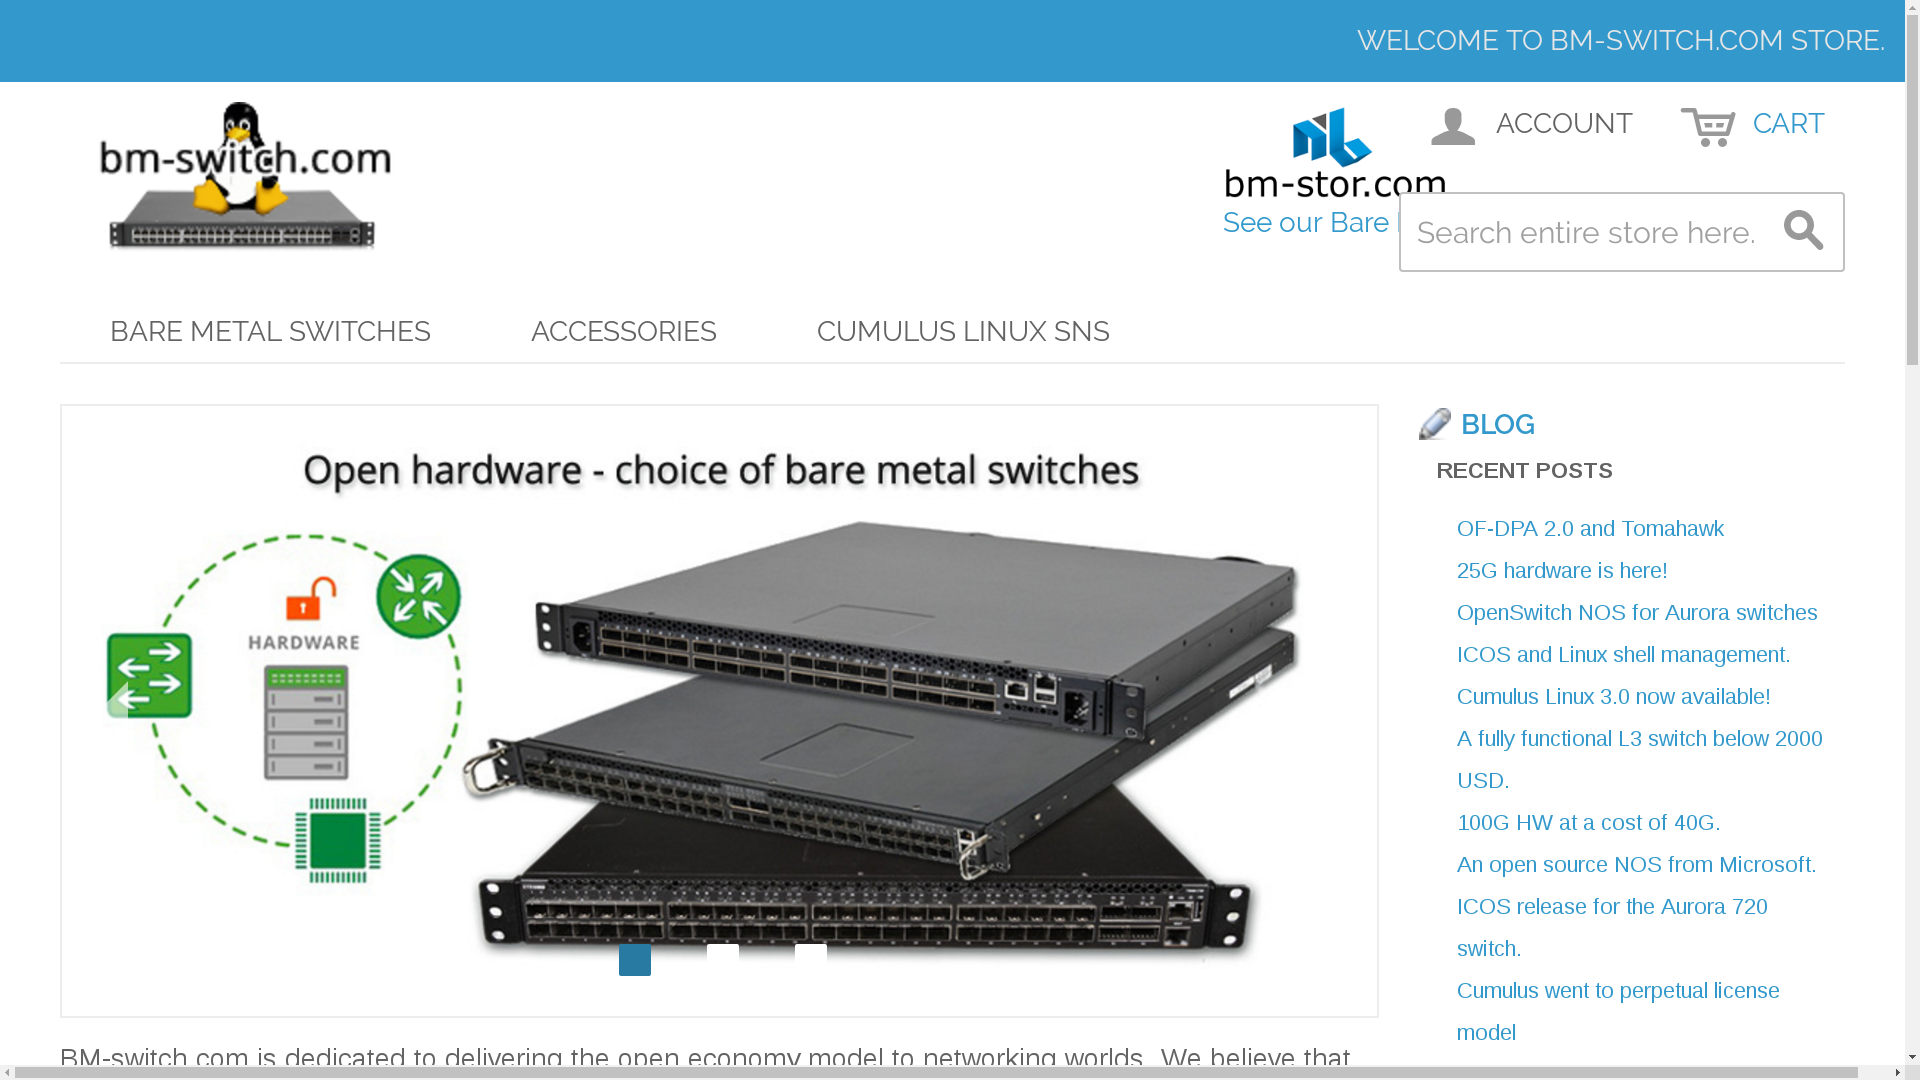
\includegraphics[keepaspectratio=true,height=1.10\textheight,width=1.00\textwidth,angle=0]{www-bm-switch.png}
 \caption{Bare Metal Switches Website}
 \label{fig:www-bm-switch}
\end{figure}

\subsection{Colfax Direct}


\begin{figure}[h!]
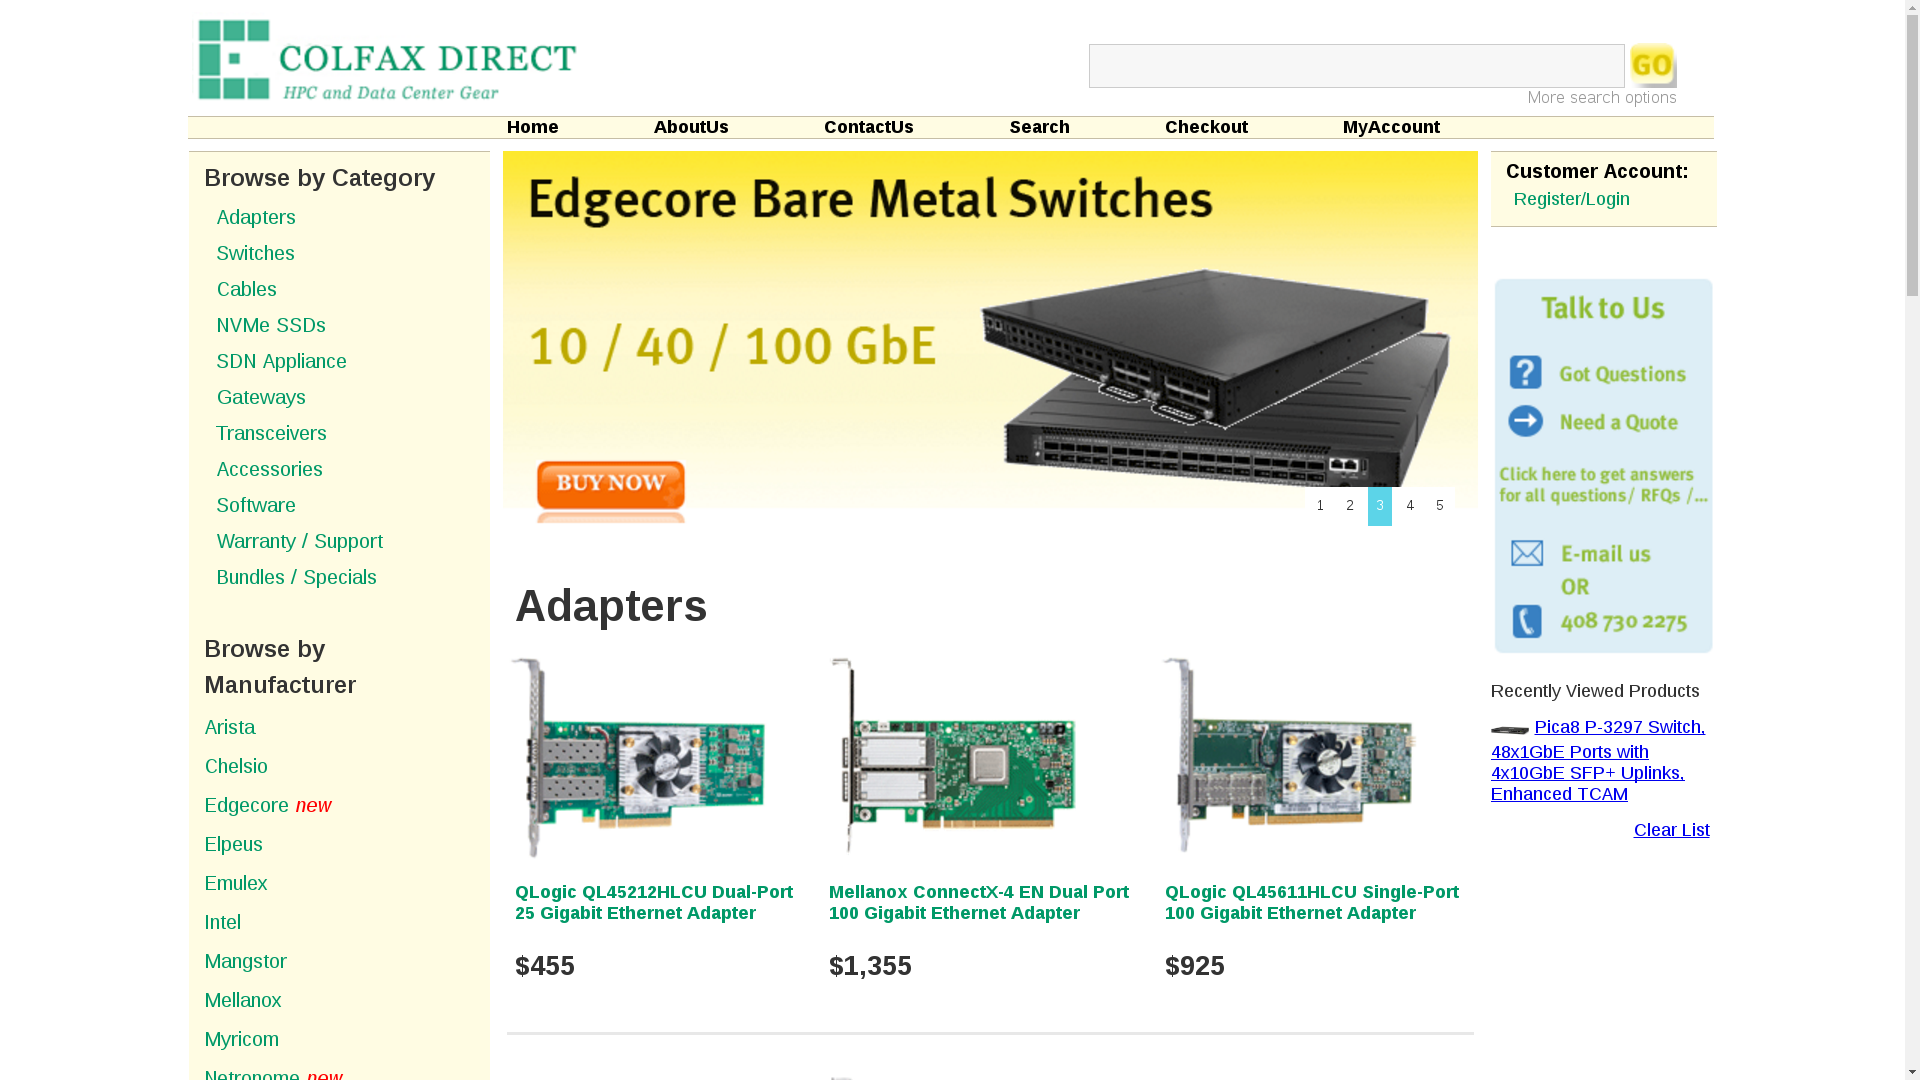
\includegraphics[keepaspectratio=true,height=1.10\textheight,width=1.00\textwidth,angle=0]{www-colfax.png}
 \caption{Colfax Direct Website}
 \label{fig:www-colfax}
\end{figure}

